\documentclass{standalone}
\usepackage{tikz}
\usetikzlibrary{shapes.geometric, arrows.meta, positioning, backgrounds, fit}

\begin{document}

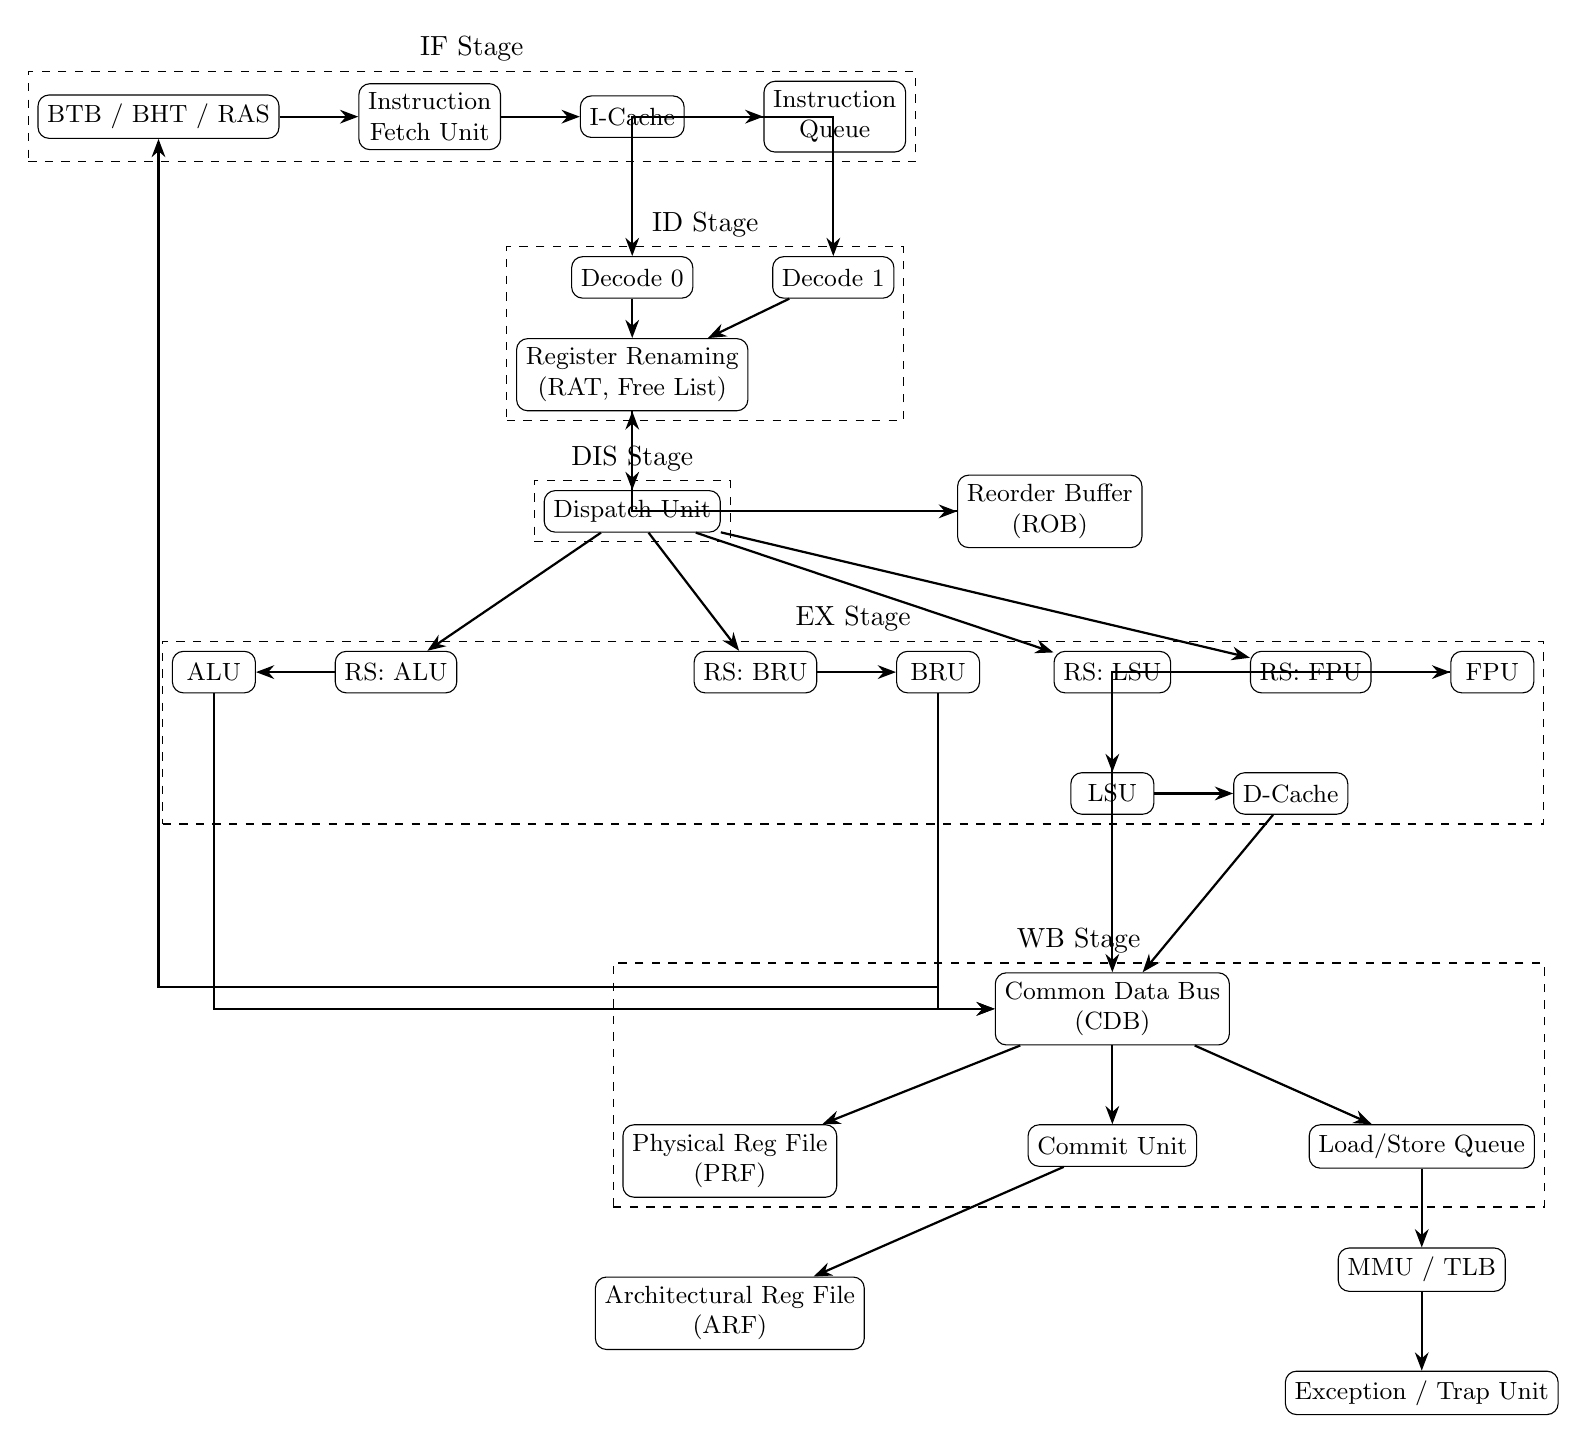
\begin{tikzpicture}[
    box/.style={rectangle, draw, rounded corners, minimum height=1.5em, minimum width=3em, align=center, font=\small},
    arrow/.style={-Stealth, thick},
    node distance=1cm and 1cm
]

% Nodes (Define all nodes first)
% IF Stage Nodes
\node[box] (btb) at (0, 0) {BTB / BHT / RAS};
\node[box, right=of btb] (ifetch) {Instruction\\Fetch Unit};
\node[box, right=of ifetch] (icache) {I-Cache};
\node[box, right=of icache] (iqueue) {Instruction\\Queue};

% ID Stage Nodes
\node[box, below=1.5cm of icache] (decode0) {Decode 0};
\node[box, right=of decode0] (decode1) {Decode 1};
\node[box, below=0.5cm of decode0] (rename) {Register Renaming\\(RAT, Free List)};

% DIS Stage Nodes
\node[box, below=1cm of rename] (dispatch) {Dispatch Unit};
\node[box, right=3cm of dispatch] (rob) {Reorder Buffer\\(ROB)};

% EX Stage Nodes
\node[box, below=1.5cm of dispatch, xshift=-3cm] (rs_alu) {RS: ALU};
\node[box, left=of rs_alu] (alu) {ALU};
\node[box, right=3cm of rs_alu] (rs_bru) {RS: BRU}; % Adjusted position to avoid overlap
\node[box, right=of rs_bru] (bru) {BRU};
\node[box, right=3cm of rs_bru] (rs_lsu) {RS: LSU}; % Adjusted position to avoid overlap
\node[box, below=of rs_lsu] (lsu) {LSU};
\node[box, right=of lsu] (dcache) {D-Cache};
\node[box, right=1cm of rs_lsu] (rs_fpu) {RS: FPU};
\node[box, right=of rs_fpu] (fpu) {FPU};

% WB Stage Nodes
\node[box, below=2cm of lsu] (cdb) {Common Data Bus\\(CDB)};
\node[box, below left=1cm and 2cm of cdb] (prf) {Physical Reg File\\(PRF)};
\node[box, below=of cdb] (commit) {Commit Unit};
\node[box, below right=1cm and 1cm of cdb] (lsq) {Load/Store Queue};

% Memory and Exception Nodes
\node[box, below=of lsq] (mmu) {MMU / TLB};
\node[box, below=of prf] (arf) {Architectural Reg File\\(ARF)};
\node[box, below=of mmu] (trap) {Exception / Trap Unit};

% Fit boxes for pipeline stages (Defined after nodes)
\begin{scope}[on background layer]
    \node[draw, dashed, fit={(btb) (ifetch) (icache) (iqueue)}, label=above:IF Stage] {};
    \node[draw, dashed, fit={(decode0) (decode1) (rename)}, label=above:ID Stage] {};
    \node[draw, dashed, fit={(dispatch)}, label=above:DIS Stage] {};
    \node[draw, dashed, fit={(rs_alu) (alu) (rs_bru) (bru) (rs_lsu) (lsu) (dcache) (rs_fpu) (fpu)}, label=above:EX Stage] {};
    \node[draw, dashed, fit={(cdb) (prf) (commit) (lsq)}, label=above:WB Stage] {};
\end{scope}

% Arrows
\draw[arrow] (btb) -- (ifetch);
\draw[arrow] (ifetch) -- (icache);
\draw[arrow] (icache) -- (iqueue);
\draw[arrow] (iqueue) -| (decode0);
\draw[arrow] (iqueue) -| (decode1);
\draw[arrow] (decode0) -- (rename);
\draw[arrow] (decode1) -- (rename);
\draw[arrow] (rename) -- (dispatch);
\draw[arrow] (dispatch) -- (rs_alu);
\draw[arrow] (dispatch) -- (rs_bru);
\draw[arrow] (dispatch) -- (rs_lsu);
\draw[arrow] (dispatch) -- (rs_fpu);
\draw[arrow] (dispatch) -- (rob);
\draw[arrow] (rs_alu) -- (alu);
\draw[arrow] (rs_bru) -- (bru);
\draw[arrow] (rs_lsu) -- (lsu);
\draw[arrow] (lsu) -- (dcache);
\draw[arrow] (rs_fpu) -- (fpu);
\draw[arrow] (alu) |- (cdb);
\draw[arrow] (bru) |- (cdb);
\draw[arrow] (dcache) -- (cdb);
\draw[arrow] (fpu) -| (cdb);
\draw[arrow] (cdb) -- (prf);
\draw[arrow] (cdb) -- (commit);
\draw[arrow] (cdb) -- (lsq);
\draw[arrow] (lsq) -- (mmu);
\draw[arrow] (commit) -- (arf);
\draw[arrow] (mmu) -- (trap);

% Feedback loops
\draw[arrow] (bru) |- ++(-2, -4) -| (btb); % Feedback to BTB
\draw[arrow] (rob) -| (rename);

\end{tikzpicture}

\end{document}